\documentclass[titlepage]{article}
\usepackage{fullpage}
\usepackage{graphics,indentfirst,amsmath,amsthm,amssymb,latexsym,enumerate}
\usepackage{graphicx}
\begin{document}

\title{17-651 Models of Software Systems\\[1ex] Project 2: Concurrency}
\author{
{\Large\textbf{Group 9}}\\[3ex]
Ajay Nair\\[1ex] Huairui Qi\\[1ex] Yu-Chun Shih\\[1ex] Nianjie Wan\\[1ex]Songbo Wu}
\date{\today}
\maketitle

\section{Modeling with Concurrency}

    \subsection{Assumption}
    \begin{enumerate}
        \item If both the AC power and the battery fails, the power system of the infusion pump will fail.\\
        The user manual suggests that there are only two power sources in the infusion pump: AC power and the battery. Therefore, we assume that if the AC power is failed and the battery is not working as well, the whole power system will go down.
        \item The pump cannot be turned off if the pump is running an infusion.\\
        For safety reasons, the pump must not be turned off if the pump is running an infusion. The user manual implicitly stated that when the user switches off the pump, the front door of the pump must be closed and any infusion must be on hold. Therefore, we came up with the assumption that when the pump is in the infusion state, turning off the pump may not be an option.
        \item The action \texttt{purge\_air} and \texttt{lock\_line} is done automatically and sequentially by the system which are hided from the user.\\
        For safety issues, the pump must purge the air inside the infusion line to make sure that there is no bubble inside. The line will be locked automatically afterward. We assume that these two actions will be done systematically and automatically without any interaction with the user or nurses.
    \end{enumerate}
    
    \subsection{Abstraction}
    \begin{enumerate}
        \item User input abstraction\\
        In the user manual, there is a component on the user interface where the user can set the rate and volume of the medicine in the infusion pump. However, we do not model the actual number that the user set in our model. We turn it into an abstraction with only one action \texttt{set\_rate} and \texttt{enter\_value} instead of the actual number to prevent over-complexity in our system.
        \item Alarm abstraction\\
        In the user manual, we can see that there three different types of alarm, which are insistent, non-insistent and continuous alarm. However, we abstracted away from these different type of alarm and made it into one single alarm that will sound whenever the infusion line break. Moreover, although we have two different infusion lines that run concurrently in our model, our model abstracted from the real world infusion pump and states that all of the infusion lines will be sharing one single alarm. Therefore the alarm will sound whenever there is a line break.
        \item Components communication abstraction.\\
        In the real system, after the user presses a button on UI, for example, turn off button, the UI would send a signal to the power system and the power system would call some function to turn off the machine. However, in our model, we abstract away the communication that happens after the interaction between the user and UI. In other words, although the button on the user interface may break and the communication between UI and other components of the system may fail, we assume that in our model, if turn on or turn off button is pressed, the power system will perform the same action accordingly without any failure. As a result, actions like \texttt{turn\_on} are used directly to synchronize different processes.
    \end{enumerate}
    
    \subsection{High-level Overview}
        Our model has concurrent processes of the power system, two lines, one alarm, and two user interfaces. The power system and the alarm is shared by both lines, and each line has its own user interfaces.  
   
        \begin{enumerate}
            \item The power system uses both electricity and backup battery. If one of the sources fails, the other process will keep working and if both fail, then the system will fail.
            \item For the working process of lines, users need to set the parameter first and then connect and lock the line to start the infusion process. If something wrong happens with the lines, the system will notify the alarm.
            \item The alarm will sound when there are errors happening in the system. And the users can mute the alarm manually or fix the errors to mute the alarm. While multiple errors occur, the alarm would be muted automatically only when all the errors are fixed.
            \item The user interface contains all the actions users can operate within the system, including turning on and turning off the system, setting the parameters of lines, dispensing the flow, confirming and canceling each decision in the line infusion process, muting the alarm, and fixing the errors on power system and lines.
        \end{enumerate}
   
    \subsection{Structure Diagram}
   
       \begin{figure}[h]
           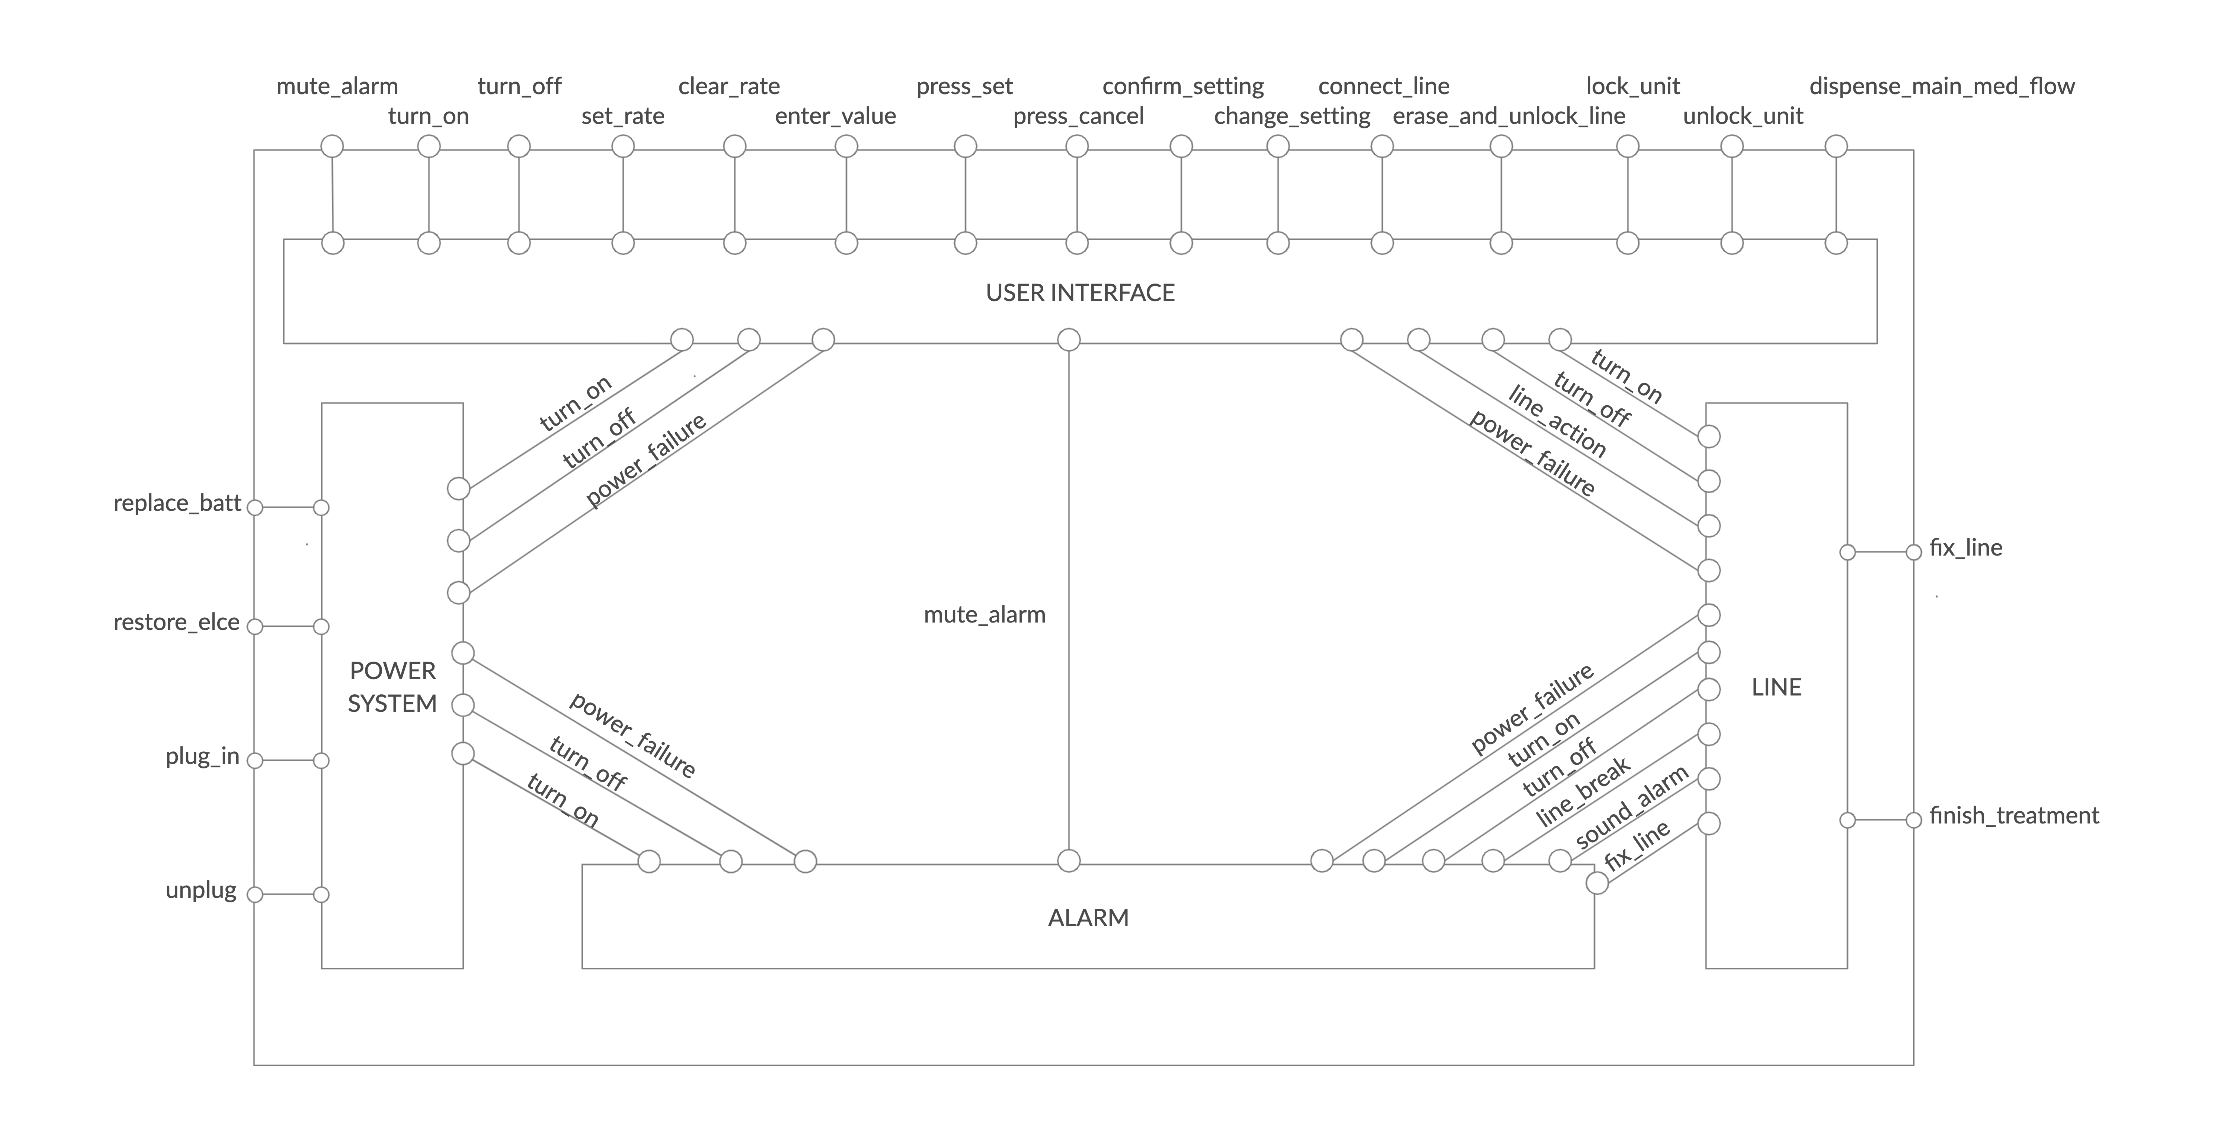
\includegraphics[width=\linewidth]{graph.jpg}
           \caption{Structure Diagram for Pump}
           \label{fig:diagram}
       \end{figure}
    
  
        \begin{enumerate}
        \item The \texttt{PUMP} FSP exposes all the actions in the \texttt{UserControlMenu} which can be performed by the user in real life. And hides all the other actions used by processes to communicate with each other.
        
        \item All of the four major components, namely \texttt{USER\_INTERFACE}, \texttt{LINE}, \texttt{ALARM} , \texttt{POWER\_SYSTEM}, share actions \texttt{turn\_on}, \texttt{turn\_off}, \texttt{power\_failure}.
        
        \item The major component process \texttt{USER\_INTERFACE} exposes all the actions the user can perform on the control panel of the infusion pump. According to the components communication abstraction we made, some actions like \texttt{turn\_on} are shared between \texttt{UI} and \texttt{LINE}, \texttt{UI} and \texttt{POWER\_SYSTEM}, etc. It's the same case with other actions represented by \texttt{line\_actions}, namely,
        
        \texttt{set\_rate, enter\_value, press\_set. press\_cancel, clear\_rate, connect\_line, confirm\_setting, erase\_and\_unlock\_line}.
        
        \item \texttt{POWER\_SYSTEM} contains and exposes physical actions of the user like \texttt{replace\_batt}, \texttt{restore\_elec}, \texttt{plug\_in}, and \texttt{unplug}. As the name suggests, the actions are physical actions performed by the user to change the status of the power system.
        
        \item \texttt{LINE} and \texttt{ALARM} share actions \texttt{line\_break}, \texttt{sound\_alarm} to simulate the error happens in the infusion pump. The physical action \texttt{fix\_line} is performed by the user to fix the broken line.
        
        \item \texttt{USER\_INTERFACE} and \texttt{ALARM} share only one action \texttt{mute\_alarm}, which is a button to mute the alarm on the user interface.
    \end{enumerate}

\section{Properties}
\begin{verbatim}
    // Settings will be confirmed after confirming the settings event until the settings
    // are confirmed or power failure or when the system is turned off
    fluent CONFIRM_SETTING[i:LineIDs] = <line[i].confirm_settings,
        {line[i].change_settings, turn_off, power_failure}> 
        initially False
 
    // The system will be pumping after dispensing the flow until 
    // a line break or until we unlock the unit or until we turn off 
    // the system or there is a power failure (battery and AC)
    fluent PUMPING[i:LineIDs] = <line[i].dispense_main_med_flow,
        {line[i].line_break, line[i].unlock_unit, turn_off, power_failure}>
        initially False
        
    // Electrical failure happens after the system is unplugged or until 
    // there is an electrical failure
    fluent ELEC_FAILURE = <{unplug, elec_failure}, plug_in> 
        initially True
    
    // Battery failure is true after the battery fails until the battery is replaced
    fluent BATT_FAILURE = <batt_failure, replace_batt> 
        initially False

    // Power failure is true after power fails and either the battery is replaced or
    // electricity is plugged in
    fluent POWER_FAILURE = <power_failure, {replace_batt, plug_in}> 
        initially False
    
    // Line failure is true after a line break until the line is fixed
    fluent LINE_FAILURE[i:LineIDs] = <line[i].line_break, {line[i].fix_line}>
        initially False
        
    // Alarm is sounding after alarm sounds until it is either stopped or muted or
    // if the system is turned off or there is a power failure
    fluent ALARM_SOUND = <alarm_sound, {alarm_stop, turn_off, power_failure, mute_alarm}>
        initially False
    
    // Alarm is stopped after the alarm is stopped or after a power failure or 
    // after the system is turned off until the alarm sound is on again
    fluent ALARM_STOPPED = <{alarm_stop, power_failure, turn_off}, alarm_sound>
        initially True
    
    // Alarm is muted after the alarm is muted until it sounds again on 
    // the system is turned off or there is a power failure
    fluent ALARM_MUTED = <mute_alarm, {alarm_stop, alarm_sound, turn_off, power_failure}>
        initially True
    
    // Unit is locked after the unit is locked until the unit is unlocked
    // or a power failure or the system is turned off
    fluent UNIT_LOCKED[i:LineIDs] = <line[i].lock_unit, 
        {line[i].unlock_unit, power_failure, turn_off}>
        initially False
    
    // The treatment is finished after the finish_treatment event 
    // until the medicine is dispensed again
    fluent TREATMENT_FINISHED[i:LineIDs] = <line[i].finish_treatment,
        {line[i].dispense_main_med_flow}>
        initially False
\end{verbatim}

\textbf{Note}: On the 3rd slide of 20 Concurrency Reasoning, it says "safety property asserts that something bad never happens". But the formal definition on the next slide says nothing about whether predicate $p$ is bad or good. There seem to be some ambiguities, so we decide to treat all the properties that assert that something always happens as safety properties and similarly with liveness properties.

\begin{enumerate}
\item The pump cannot start pumping without the operator first confirming the settings on the pump.
    \begin{itemize}
        \item Our interpretation: if pumping has started should, the settings on the pump must be confirmed already.
        \item It is true of our model. Our models allow us to check the property using the FLTL check in LSTA with fair choices.
        \item This is a safety property because it requires that pumping should never happen before the settings confirmation.
        \begin{verbatim}
assert CONFIRM_BEFORE_PUMP = [] forall[i:LineIDs] (
    PUMPING[i] -> CONFIRM_SETTING[i]
)
        \end{verbatim}
    \end{itemize}
\item Electrical power can fail infinitely often.
    \begin{itemize}
        \item This property is tricky because it uses the word "can". It's not saying that the electrical power fails infinitely often, instead, it's saying that the power could fail infinitely often. We don't think the property can be accurately modeled by FLTL, so we modified this into that the electrical power fails infinitely often.
        \item It is true of our model. Our models allow us to check the property using the FLTL check in LSTA with fair choices.
        \item The original version is neither safety nor liveness property because it's saying that some bad \textbf{could} happen infinitely often. However, it's also disputable for the modified version because it's a progress property that says that something \textbf{bad} happens infinitely often.
\begin{verbatim}
assert ELEC_FAILS_INFINITELY = []<> ELEC_FAILURE
\end{verbatim}
    \end{itemize}

\item If the backup battery power fails, pumping will not occur on any line.
    \begin{itemize}
    \item Our model does not follow this property by design. In the system that we modeled, there are 2 types of power source: 
    1. AC power
    2. Battery backup power\\
    When the AC power fails we switch to battery and then if the AC power is back then we switch to AC. When the backup battery fails, it does not necessarily means that the AC power is also failed. In our model, the pumping will not occur on any line when both the AC power and the battery is failed.
    \item This is a safety property because it requires pumping never happens if the backup battery power fails.
    \begin{verbatim}
assert BATT_FAILS_THEN_STOP_PUMPING = [] (BATT_FAILURE ->
    forall[i:LineIDs] (!PUMPING[i]))
    \end{verbatim}
 \end{itemize}

\item It is always possible to resume pumping after a failure.
    \begin{itemize}
        \item Our interpretation: after power or line failure the model should be able to reach pumping state sometime in the future eventually
        \item It is true of our model. Our models allow us to check the property using the FLTL check in LSTA with fair choices.
        \item This is a liveness property. 
        Because in each state of the infusion pump model, this requires when there is a failure appears(either \texttt{power\_failure} or \texttt{line\_failure}), the error should eventually be fixed and the infusion pump would resume pumping again.
        \begin{verbatim}
assert RESUME_AFTER_FAILURE = [] forall[i:LineIDs] (
    (POWER_FAILURE || LINE_FAILURE[i]) -> <> PUMPING[i]
)
        \end{verbatim}
    \end{itemize}

\item An alarm will sound on any line failure.
    \begin{itemize}
        \item Our model does not follow this property by design. We have modeled the system such that alarm will sound once there is any failure. But both lines run in parallel and failure in one line does not have any effect on the other line. So when line 1 fails it is possible for other actions to happen in line 2. Thus we cannot state the rule that alarm should be the next state after failure. Moreover, we also cannot say that alarm will eventually sound as it may sound for some other future failure too.
        \item This is a liveness property because alarm sounding on line failure is useful to the system. What we don't want is that the alarm fails to detect the failure and to alert the user.
            \begin{verbatim}
assert ALARM_IF_LINE_FAILS = [] forall[i:LineIDs] (
    LINE_FAILURE[i] -> X ALARM_SOUND
)
            \end{verbatim}
    \end{itemize}

\item In the absence of errors the pump will continue to pump until the treatment is finished.
    \begin{itemize}
        \item Our interpretation: the description of the property is confusing in the sense that it uses the word "continue". As a result, the pumping should be already pumping at some point before it "continues" to pump. We resolve the ambiguity by modifying it into the following property: if there's no errors and the unit is locked till the treatment is finished, the pump is pumping until the treatment is finished.
        \item It is true of our model. Our models allow us to check the property using the FLTL check in LSTA with fair choices.
        \item The modified version is a safety property because it requires that the property should \textbf{always} hold under a certain condition.
            \begin{verbatim}
assert CONTINUE_PUMPING_IF_NO_ERROR = [] forall[i:LineIDs] (
PUMPING[i] -> (
        (!(POWER_FAILURE || LINE_FAILURE[i]) && UNIT_LOCKED[i] U 
            TREATMENT_FINISHED[i])
        -> (PUMPING[i] U TREATMENT_FINISHED[i])
    )
)
            \end{verbatim}
        \end{itemize}
        
\item The system never deadlocks. (Tested automatically.)
    \begin{itemize}
        \item It is true of our model. LTSA tests it by default when we compile our model. Deadlock: No action in the model results in that it reaches a state in which it cannot continue.
        \item This is a safety property because it requires that the system \textbf{never} deadlocks.
    \end{itemize}

\item Once activated, alarm sounds infinitely often until muted or stopped.
    \begin{itemize}
        \item Our interpretation: our system models alarm such that it can either be muted or stopped.
        \item It is true of our model. Our models allow us to check the property using the FLTL check in LSTA with fair choices.
        \item This is a liveness property (progress property specifically) because it requires that the alarm should sound infinitely often (something useful) until muted or stopped.
            \begin{verbatim}
assert ALARM_SOUND_INFINITELY_OFTEN_UNTIL_DEALT = ([](!ALARM_STOPPED &&
    !ALARM_MUTED) -> []<>ALARM_SOUND)
            \end{verbatim}
        \end{itemize}

\item Eventually the treatment would be finished.
    \begin{itemize}
        \item Our interpretation: for all treatment, it will finish eventually.
        \item It is true of our model. Our models allow us to check the property using the FLTL check in LSTA with fair choices.
        \item This is a liveness property because it requires the treatment eventually finishes.
            \begin{verbatim}
assert TREATMENT_FINISH_EVENTUALLY = forall[i:LineIDs] (
    <> TREATMENT_FINISHED[i]
)
            \end{verbatim}
    \end{itemize}

\end{enumerate}
\section{Reflection}

\subsection{Pre-Post Conditions}

Pre-conditions and post-conditions provide us a concise way to specify the intended requirements of the system. We can use the pre-conditions to specify what it takes for the transition to occur and we can use the post-conditions to specify what are the effects of the transition that has been taken. It could be very useful in the initial phase of design because it helps the designer to specify the behaviors of the system in mathematical form, which is concise and precise. We would recommend using this notation to formulate the idea at the beginning of the design process.

However, this notation sometimes becomes too concise to include relevant details, for example, the following specification represents a function that solves the integral of $\frac{e^t}{t}$:

\begin{align*}
solve(y: \mathcal{R}) & \\
   pre & \ y > 0 \\
  post & \int_{0}^{x'} \frac{e^t}{t} dt = y  \\
\end{align*}

The function \texttt{solve} has a clear goal - to find $x'$ that makes $\int_{0}^{x'} \frac{e^t}{t} dt = y$, where $y$ is the input. The specification tells us nothing about how to solve this equation to get the value of $x'$. In fact, this integral function is not even an elementary function. From this perspective, we would not recommend using this notation if you want to examine the details of the post-condition or the implementation of how to achieve the post condition.

We found that sometimes it seems to be a arbitrary choice regarding how to distribute the requirements into pre and post conditions. For example, you can move all the pre conditions to the post condition easily by using the $x$ and $x'$ notation. Although this feature gives the designers more freedom, we think it would be better to set up a standard convention for it so that the design could be easier to understand from the perspectives of different designers.

\subsection{Alloy}
Alloy is a declarative language based on relational logic. It pursues a balance between expressiveness and analyzability. Along with the language, Alloy Analyzer also provides means to check properties, to find counterexamples, and to check over-constraints. Alloy could be very useful in verifying system design such as database design, protocol design, etc. Alloy allows us to keep the high-level abstraction and to hide the implementation details. I would recommend using Alloy to verify the critical parts of the high-level system design such as internet protocols.

As pre-post conditions notation, Alloy is not designed to verify the overwhelming details of the software implementations. For example, if you want to understand why your implementation of the \text{malloc} function in C standard library keeps crashing, you wouldn't want to model your code using Alloy to do this. Instead, you can use Alloy to verify the idea of \textit{explicit list} is valid. We think it would be really helpful if the Alloy Analyzer could identify the line of code that the counterexample violates in checking assertions. During project 1, even though the analyzer gave the counterexamples, we often ended up spending a lot of time identifying the problem because the counterexample sometimes got fairly complicated.

For the Alloy notation, we found it not very intuitive to define the relations in the signature because although it seems to be a attribute to the signature, it actually is a global table that is accessible anywhere in the code. We think that it would be helpful if Alloy supports access control for this part.

\subsection{FSP (LTSA)}

FSP is a language designed to specify the behavior of concurrent systems. We can tell this from the syntax of this language - \texttt{process}, which is a widely used term in operating systems. It comes with the tool LTSA, whose last update was in June 2006. The tool is specifically designed for FSP programming language. The tool can help to check deadlocks and property violations including progress and FLTL properties. We would recommend using FSP and LTSA if you want to model critical parts of concurrent systems, such as internet communication protocols.

However, FSP and LTSA has not been updated for a long time, and the documentation or community support is quite poor compared to Alloy. As a result, the language doesn't support many features that are commonly used in modern programming languages such as nested \texttt{if} statement. Besides, like many other formal languages, it is not suitable to model details of large systems. So we wouldn't recommend using it if you want to model single-process programs that have complex business logic or the details of concurrent programs.

We think the first future development should be expanding the syntax of FSP by adding some language features such as nested \texttt{if} statement, etc. This suggestion may seem to be pretty trivial at the first glance, but it can be fairly important for the developers to decide whether to use the language or not because may software developers might just back off once they find themselves struggling with syntax and unable to get help because of the lack of documentation.

\section{FSP Model}

\begin{verbatim}
const MaxLineNum = 2
range LineIDs = 1 .. MaxLineNum

menu UserControlMenu = {
  // POWER_SYSTEM UI
  turn_on,  turn_off,
  
  // PUMP UI
  line[i:LineIDs].set_rate, line[i:LineIDs].clear_rate, line[i:LineIDs].change_settings,
  line[i:LineIDs].confirm_settings, line[i:LineIDs].dispense_main_med_flow,
  line[i:LineIDs].enter_value, line[i:LineIDs].erase_and_unlock_line,
  line[i:LineIDs].lock_unit, line[i:LineIDs].press_cancel, 
    line[i:LineIDs].press_set, line[i:LineIDs].unlock_unit,
  line[i:LineIDs].mute_alarm, line[i:LineIDs].connect_line, line[i:LineIDs].finish_treatment,

  // Physical Actions
  plug_in, unplug, replace_batt, restore_elec, // POWER_SYSTEM
  line[i:LineIDs].fix_line // PUMP
}

//=====================
// Power System Process 
//=====================

const ElecBroken = 0
const ElecWorking = 1
range ElecStateT = ElecBroken .. ElecWorking

const Unplugged = 0
const Plugged = 1
range PlugStateT = Unplugged .. Plugged

const BattBroken = 0
const BattWorking = 1
range BattStateT = BattBroken .. BattWorking

const PowerOff = 0
const PowerOn = 1
range PowerStateT = PowerOff .. PowerOn

POWER_SYSTEM = SUB_POWER_SYSTEM[ElecWorking][Unplugged][BattWorking][PowerOff],
SUB_POWER_SYSTEM[elec:ElecStateT][plug:PlugStateT][batt:BattStateT][power:PowerStateT] = (
  // The power system is able to be turned on
  when (power == PowerOff && (batt == BattWorking || (elec == ElecWorking && plug == Plugged)))
    turn_on -> SUB_POWER_SYSTEM[elec][plug][batt][PowerOn]
  |
  // The power system is already working - supplied by either sources
  when (power == PowerOn)
    turn_off -> SUB_POWER_SYSTEM[elec][plug][batt][PowerOff]
  |
  // The power is supplied by both, when unplug the pump, battery still stays the same
  when (power == PowerOn && batt == BattWorking && elec == ElecWorking && plug == Plugged)
    unplug -> SUB_POWER_SYSTEM[elec][Unplugged][batt][PowerOn]
  |
  // When electric failure occurs, the battery still stays the same
  when (power == PowerOn && batt == BattWorking && elec == ElecWorking && plug == Plugged)
    elec_failure -> SUB_POWER_SYSTEM[ElecBroken][plug][batt][PowerOn]
  |
  // When battery failure occurs, the electricity still stays the same
  when (power == PowerOn && batt == BattWorking && elec == ElecWorking && plug == Plugged)
    batt_failure -> SUB_POWER_SYSTEM[elec][plug][BattBroken][PowerOn]
  |
  // The power is supplied solely by electricity
  when (power == PowerOn && batt == BattBroken && elec == ElecWorking && plug == Plugged)
    unplug -> power_failure -> SUB_POWER_SYSTEM[elec][Unplugged][batt][PowerOff]
  |
  when (power == PowerOn && batt == BattBroken && elec == ElecWorking && plug == Plugged)
    power_failure -> SUB_POWER_SYSTEM[ElecBroken][plug][batt][PowerOff]
  |
  // The power is supplied solely by the battery
  when (power == PowerOn && batt == BattWorking && (elec == ElecBroken || plug == Unplugged))
    power_failure -> SUB_POWER_SYSTEM[elec][plug][BattBroken][PowerOff]
  |
  // The battery is not working properly
  when (batt == BattBroken)
    // Replace the battery
    replace_batt -> SUB_POWER_SYSTEM[elec][plug][BattWorking][power]
  |
  // The cord is unplugged
  when (plug == Unplugged)
    // Plug in the cord
    plug_in -> SUB_POWER_SYSTEM[elec][Plugged][batt][power]
  |
  // The external electricity is broken
  when (elec == ElecBroken)
    // Restore the external electricity
    restore_elec -> SUB_POWER_SYSTEM[ElecWorking][plug][batt][power]
).

//=====================
// Line Process 
//=====================


const LineBroken = 0
const LineWorking = 1
range LineStateT = LineBroken .. LineWorking

//
// States of the pump settings
//
const ParamsNotSet = 0    // pump parameters not set yet
const ParamsSet    = 1    // pump parameters already set
range ParamsStateT = ParamsNotSet .. ParamsSet

//
// Locked/unlocked states of a line with respect to a pump channel
//
const LineUnlocked = 0  // line not locked into a pump channel 
const LineLocked   = 1  // line locked into a pump channel
range LineLockStateT = LineUnlocked .. LineLocked

//
// Locked/unlocked states of the pump unit
//
const UnitUnlocked = 0  // the keypad of the pump is not locked
const UnitLocked   = 1  // the keypad of the pump is locked
range UnitLockStateT = UnitUnlocked .. UnitLocked

LINE = LINE_OFF,
LINE_OFF = (
  turn_on -> LINE_SETUP[ParamsNotSet][LineWorking][LineUnlocked]
),

//
// Line in setup mode:
// - Once required line parameters (just rate in this case) are set,
//   physical connections can be made and line can be locked
//
LINE_SETUP[params:ParamsStateT][state:LineStateT][lock:LineLockStateT] = (
  // Line will be off when the pump is not working
  power_failure -> LINE_OFF
  |
  turn_off -> LINE_OFF
  |
  // The line is broken, then fix the line
  when (state == LineBroken)
    fix_line -> LINE_SETUP[params][LineWorking][lock]
  |
  // The line could broken at any time
  when (state == LineWorking)
    line_break -> LINE_SETUP[params][LineBroken][lock]
  |
  // When parameters have not been set, user can choose the set the value
  when (params == ParamsNotSet && state == LineWorking && lock == LineUnlocked)
    set_rate -> enter_value ->
            (press_set -> LINE_SETUP[ParamsSet][state][lock]
             |
             press_cancel -> LINE_SETUP[ParamsNotSet][state][lock])
  |
  // The rate can be cleared after being set
  when (params == ParamsSet && state == LineWorking && lock == LineUnlocked)
        clear_rate -> LINE_SETUP[ParamsNotSet][state][lock]
    |
    // Connect and lock line to setup the line after setting the rate
    when (params == ParamsSet && state == LineWorking && lock == LineUnlocked)
        connect_line -> purge_air -> lock_line -> LINE_SETUP[params][state][LineLocked]
    |
    // Confirm the settings to start infusion
    when (params == ParamsSet && state == LineWorking && lock == LineLocked)
        confirm_settings -> LINE_INFUSION[UnitUnlocked]
    |
    // Unlock the line to set the value again
    when (params == ParamsSet && state == LineWorking && lock == LineLocked)
        erase_and_unlock_line -> LINE_SETUP[params][state][LineUnlocked]
),

//
// Line in infusion mode:
// - Always be able to turn the line off, even if locked
// - Allow the user to lock/unlock the unit
// - Errors could occur with the line (e.g., line became pinched or plugged)
//
LINE_INFUSION[unitLock:UnitLockStateT] = (
  // Power failure will shut down the infusion
  power_failure -> LINE_OFF
  |
  // Infusion line can be turned off
  when (unitLock == UnitUnlocked)
    turn_off -> LINE_OFF
  |
  // If the line errors occur, the alarm will sound
  line_break -> sound_alarm -> LINE_SETUP[ParamsSet][LineBroken][LineUnlocked]
  |
  // If the unit is not locked, it can change the setting
  when (unitLock == UnitUnlocked)
        change_settings -> LINE_SETUP[ParamsSet][LineWorking][LineLocked]
    |
    // Lock unit if it is unlocked
    when (unitLock == UnitUnlocked)
        lock_unit -> LINE_INFUSION[UnitLocked]
    |
    // Unlock unit if it is locked
    when (unitLock == UnitLocked)
        unlock_unit -> LINE_INFUSION[UnitUnlocked]
  |
  // Nurse can choose to finish the treatment
  when (unitLock == UnitLocked)
        finish_treatment -> LINE_INFUSION[UnitUnlocked]
    |
      // Nurse can choose to start dispensing the flow after locking the unit
  when (unitLock == UnitLocked)
      dispense_main_med_flow -> LINE_INFUSION[unitLock]
).


//=====================
// Alarm Process 
//=====================

//
// States of the pump alarm
//
const AlarmMuted  = 0    // Alarm currently inactive
const AlarmSounding = 1    // Alarm currently active
range AlarmStateT = AlarmMuted .. AlarmSounding

range FailedNumStateT = 0 .. MaxLineNum

// Nurses can silence the alarm even though the problem is not solved
ALARM = ALARM_POWER_OFF,
ALARM_POWER_OFF = (
  turn_on -> SUB_ALARM[AlarmMuted][0]
),
SUB_ALARM[alarmState:AlarmStateT][failedNum:FailedNumStateT] = (
  // Power off would silince the alarm
  power_failure -> ALARM_POWER_OFF
  |
  turn_off -> ALARM_POWER_OFF
  |
  // Action of alarm sounding
  when (alarmState == AlarmSounding)
    alarm_sound -> SUB_ALARM[alarmState][failedNum]
  |
  // Mute the alarm
  when (alarmState == AlarmSounding)
    mute_alarm -> SUB_ALARM[AlarmMuted][failedNum]
  |
  // If the line errors happen while the alarm already sounds, the
  // number of broken lines plus
  when (failedNum < MaxLineNum)
    line_break -> SUB_ALARM[AlarmSounding][failedNum+1]
  |
  // Fix the last line will mute the alarm, otherwise only the count of broken lines minus
  when (failedNum == 1)
    fix_line -> alarm_stop -> SUB_ALARM[AlarmMuted][failedNum-1]
  |
  when (failedNum > 1)
    fix_line -> SUB_ALARM[alarmState][failedNum-1]
).

//=====================
// User Interface
// - The actions that the user can choose to operate with in the system
//=====================

SUB_UI = UI_POWER_OFF,
UI_POWER_OFF = (
  turn_on -> UI_INIT
),
UI_INIT = (
  turn_off -> UI_POWER_OFF
  |
  power_failure -> UI_POWER_OFF
  |
  set_rate -> enter_value -> VALUE_ENTERED
),
VALUE_ENTERED = (
  turn_off -> UI_POWER_OFF
  |
  power_failure -> UI_POWER_OFF
  |
  press_cancel -> UI_INIT
  |
  press_set -> VALUE_SET
),
VALUE_SET = (
  turn_off -> UI_POWER_OFF
  |
  power_failure -> UI_POWER_OFF
  |
  clear_rate -> UI_INIT
  |
  connect_line -> LINE_CONNECTED
),
LINE_CONNECTED = (
  turn_off -> UI_POWER_OFF
  |
  power_failure -> UI_POWER_OFF
  |
  confirm_settings -> SETTING_CONFIRMED
  |
  erase_and_unlock_line -> VALUE_SET
),
SETTING_CONFIRMED = (
  turn_off -> UI_POWER_OFF
  |
  power_failure -> UI_POWER_OFF
  |
  change_settings -> LINE_CONNECTED
  |
  lock_unit -> UNIT_LOCKED
),
UNIT_LOCKED = (
  power_failure -> UI_POWER_OFF
  |
  unlock_unit -> SETTING_CONFIRMED
  |
  dispense_main_med_flow -> UNIT_LOCKED
).

//=====================
// Composed Process
//=====================

||PUMP = (line[LineIDs]:LINE || POWER_SYSTEM || {line[LineIDs]}::ALARM
  || line[LineIDs]:SUB_UI) /
  {turn_on / line[LineIDs].turn_on,
  turn_off / line[LineIDs].turn_off,
  power_failure / line[LineIDs].power_failure,
  mute_alarm / line[LineIDs].mute_alarm,
  alarm_sound / line[LineIDs].alarm_sound}.

//=====================
// Properties
//=====================

const False = 0
const True = 1

// Settings will be confirmed after confirming the settings event until the settings 
// are confirmed or power failure or when the system is turned off 
fluent CONFIRM_SETTING[i:LineIDs] = <line[i].confirm_settings,
  {line[i].change_settings, turn_off, power_failure}>
  initially False

// The system will be pumping after dispensing the flow until
// a line break or until we unlock the unit or until we turn off the system or there 
// is a power failure (battery and AC)
fluent PUMPING[i:LineIDs] = <line[i].dispense_main_med_flow,
  {line[i].line_break, line[i].unlock_unit, turn_off, power_failure}>
  initially False

// Electrical failure happens after the system is unplugged or until 
// there is an electrical failure 
fluent ELEC_FAILURE = <{unplug, elec_failure}, plug_in>
  initially True

// Battery failure is true after the battery fails until the battery is replaced
fluent BATT_FAILURE = <batt_failure, replace_batt>
  initially False

// Power failure is true after power fails and either the battery is replaced or
// electricity is plugged in
fluent POWER_FAILURE = <power_failure, {replace_batt, plug_in}>
  initially False

// Line failure is true after a line break until the line is fixed
fluent LINE_FAILURE[i:LineIDs] = <line[i].line_break, {line[i].fix_line}>
  initially False

// Alarm is sounding after alarm sounds until it is either stopped or muted or
// if the system is turned off or there is a power failure
fluent ALARM_SOUND = <alarm_sound, {alarm_stop, turn_off, power_failure, mute_alarm}>
  initially False

// Alarm is stopped after the alarm is stopped or after a power failure or 
// after the system is turned off until the alarm sound is on again
fluent ALARM_STOPPED = <{alarm_stop, power_failure, turn_off}, alarm_sound>
  initially True

// Alarm is muted after the alarm is muted until it sounds again on 
// the system is turned off or there is a power failure
fluent ALARM_MUTED = <mute_alarm, {alarm_stop, alarm_sound, turn_off, power_failure}>
  initially True

// Unit is locked after the unit is locked until the unit is unlocked
// or a power failure or the system is turned off
fluent UNIT_LOCKED[i:LineIDs] = <line[i].lock_unit, {line[i].unlock_unit,
  power_failure, turn_off}>
  initially False

// The treatment is finished after the finish_treatment event 
// until the medicine is dispensed again
fluent TREATMENT_FINISHED[i:LineIDs] = <line[i].finish_treatment,
  {line[i].dispense_main_med_flow}>
  initially False

// 1. The pump cannot start pumping without the operator first confirming the
// settings on the pump.
assert CONFIRM_BEFORE_PUMP = [] forall[i:LineIDs] (
  PUMPING[i] -> CONFIRM_SETTING[i]
)

// 2. Electrical power can fail infinitely often.
assert ELEC_FAILS_INFINITELY = []<> ELEC_FAILURE

// 3. If the backup battery power fails, pumping will not occur on any line.
// - Doesn't hold because even battery fails, it's possible that the machine
// is powered by AC power
assert BATT_FAILS_THEN_STOP_PUMPING = [] (BATT_FAILURE -> forall[i:LineIDs]
  (!PUMPING[i]))

// 4. It is always possible to resume pumping after a failure.
// (for each line.)
assert RESUME_AFTER_FAILURE = [] forall[i:LineIDs] (
  (POWER_FAILURE || LINE_FAILURE[i]) -> <> PUMPING[i]
)

// 5. An alarm will sound on any line failure.
// - Doesn't hold because it can always be interruptted.
assert ALARM_IF_LINE_FAILS = [] forall[i:LineIDs] (
  LINE_FAILURE[i] -> X ALARM_SOUND
)

// 6. In the absence of errors the pump will continue to pump until the treatment is finished.
assert CONTINUE_PUMPING_IF_NO_ERROR = [] forall[i:LineIDs] (
  PUMPING[i] -> (
    (!(POWER_FAILURE || LINE_FAILURE[i]) && UNIT_LOCKED[i] U TREATMENT_FINISHED[i])
      -> (PUMPING[i] U TREATMENT_FINISHED[i])
  )
)

// 7. The system never deadlocks. (Tested automatically.)

// 8. Alarm sound infinitely often until muted or stopped.
assert ALARM_SOUND_INFINITELY_OFTEN_UNTIL_DEALT = ([](!ALARM_STOPPED && !ALARM_MUTED)
  -> []<>ALARM_SOUND)

// 9. Eventually the treatment would be finished.
assert TREATMENT_FINISH_EVENTUALLY = forall[i:LineIDs] (
  <> TREATMENT_FINISHED[i]
)
\end{verbatim}

\end{document}